\documentclass{article}
\usepackage{amsmath,amssymb,amstext,mathtools,array,url,bm,graphicx,color,epsfig}
\usepackage{fullpage,setspace}
\usepackage{authblk}
\usepackage{filecontents}
\usepackage{natbib}
\usepackage{lineno}
\usepackage[colorlinks]{hyperref}
\usepackage{subcaption}
\usepackage{float}
\usepackage[flushleft]{threeparttable}

\def\dt{\partial t}
\def\dx{\partial x}
\def\dy{\partial y}

\def\dz{\partial z}
\def\BE{\begin{equation}}
\def\EE{\end{equation}}
\def\half{\frac{1}{2}}
\def\calT{\cal T}
\def\Deltax{\Delta x}
\def\Deltat{\Delta t}
\DeclareSymbolFont{largesymbolsA}{U}{txexa}{m}{n}
\DeclareMathSymbol{\varprod}{\mathop}{largesymbolsA}{16}

\newtheorem{theorem}{Theorem}
\newtheorem{acknowledgement}[theorem]{Acknowledgement}
\newtheorem{algorithm}[theorem]{Algorithm}
\newtheorem{axiom}[theorem]{Axiom}
\newtheorem{case}[theorem]{Case}
\newtheorem{claim}[theorem]{Claim}
\newtheorem{conclusion}[theorem]{Conclusion}
\newtheorem{condition}[theorem]{Condition}
\newtheorem{conjecture}[theorem]{Conjecture}
\newtheorem{corollary}[theorem]{Corollary}
\newtheorem{criterion}[theorem]{Criterion}
\newtheorem{definition}[theorem]{Definition}
\newtheorem{example}[theorem]{Example}
\newtheorem{exercise}[theorem]{Exercise}
\newtheorem{lemma}[theorem]{Lemma}
\newtheorem{notation}[theorem]{Notation}
\newtheorem{problem}[theorem]{Problem}
\newtheorem{proposition}[theorem]{Proposition}
\newtheorem{remark}[theorem]{Remark}
\newtheorem{solution}[theorem]{Solution}
\newtheorem{summary}[theorem]{Summary}
\newenvironment{proof}[1][Proof]{\noindent\textbf{#1.} }{\ $\square$}


\begin{document}
\title{\bf Supporting Information: Comparative anatomy of geophysical flow models and modeling assumptions using uncertainty quantification}
\author[1,3]{Abani K. Patra}
\author[2]{Andrea Bevilacqua}
\author[1]{Ali Akhavan-Safaei}
\author[4]{E. Bruce Pitman}
\author[2]{Marcus I. Bursik}
\author[2]{David Hyman}

\affil[1]{\textit{Dept. of Mech. and  Aero. Eng., University at Buffalo, Buffalo NY 14260} }
\affil[2]{\textit{Dept. of Geology, University at Buffalo, Buffalo NY 14260} }
\affil[3]{\textit{Comp. Data Science and Eng., University at Buffalo, Buffalo NY 14260} }
\affil[4]{\textit{Dept. of Materials Design and Innovation, University at Buffalo, NY, 14260}}

\date{\texttt{\{abani,abevilac,aliakhav,pitman,mib,davidhym\}@buffalo.edu}}

\maketitle
\tableofcontents
\newpage
Supporting Information includes the local plots of Froude Number, flow acceleration, and the spatial integrals of force terms.

\section{Small scale flow on inclined plane and flat runway}
\subsection{Froude Number}
Figure \ref{fig:Ramp-Fr} shows the Froude Number, $\Vert \underline{\mathbf{u}} \Vert/\sqrt{gh}$, at the points $(L_i)_{i=1,\dots,4}$.
\begin{figure}[H]
         \centering
        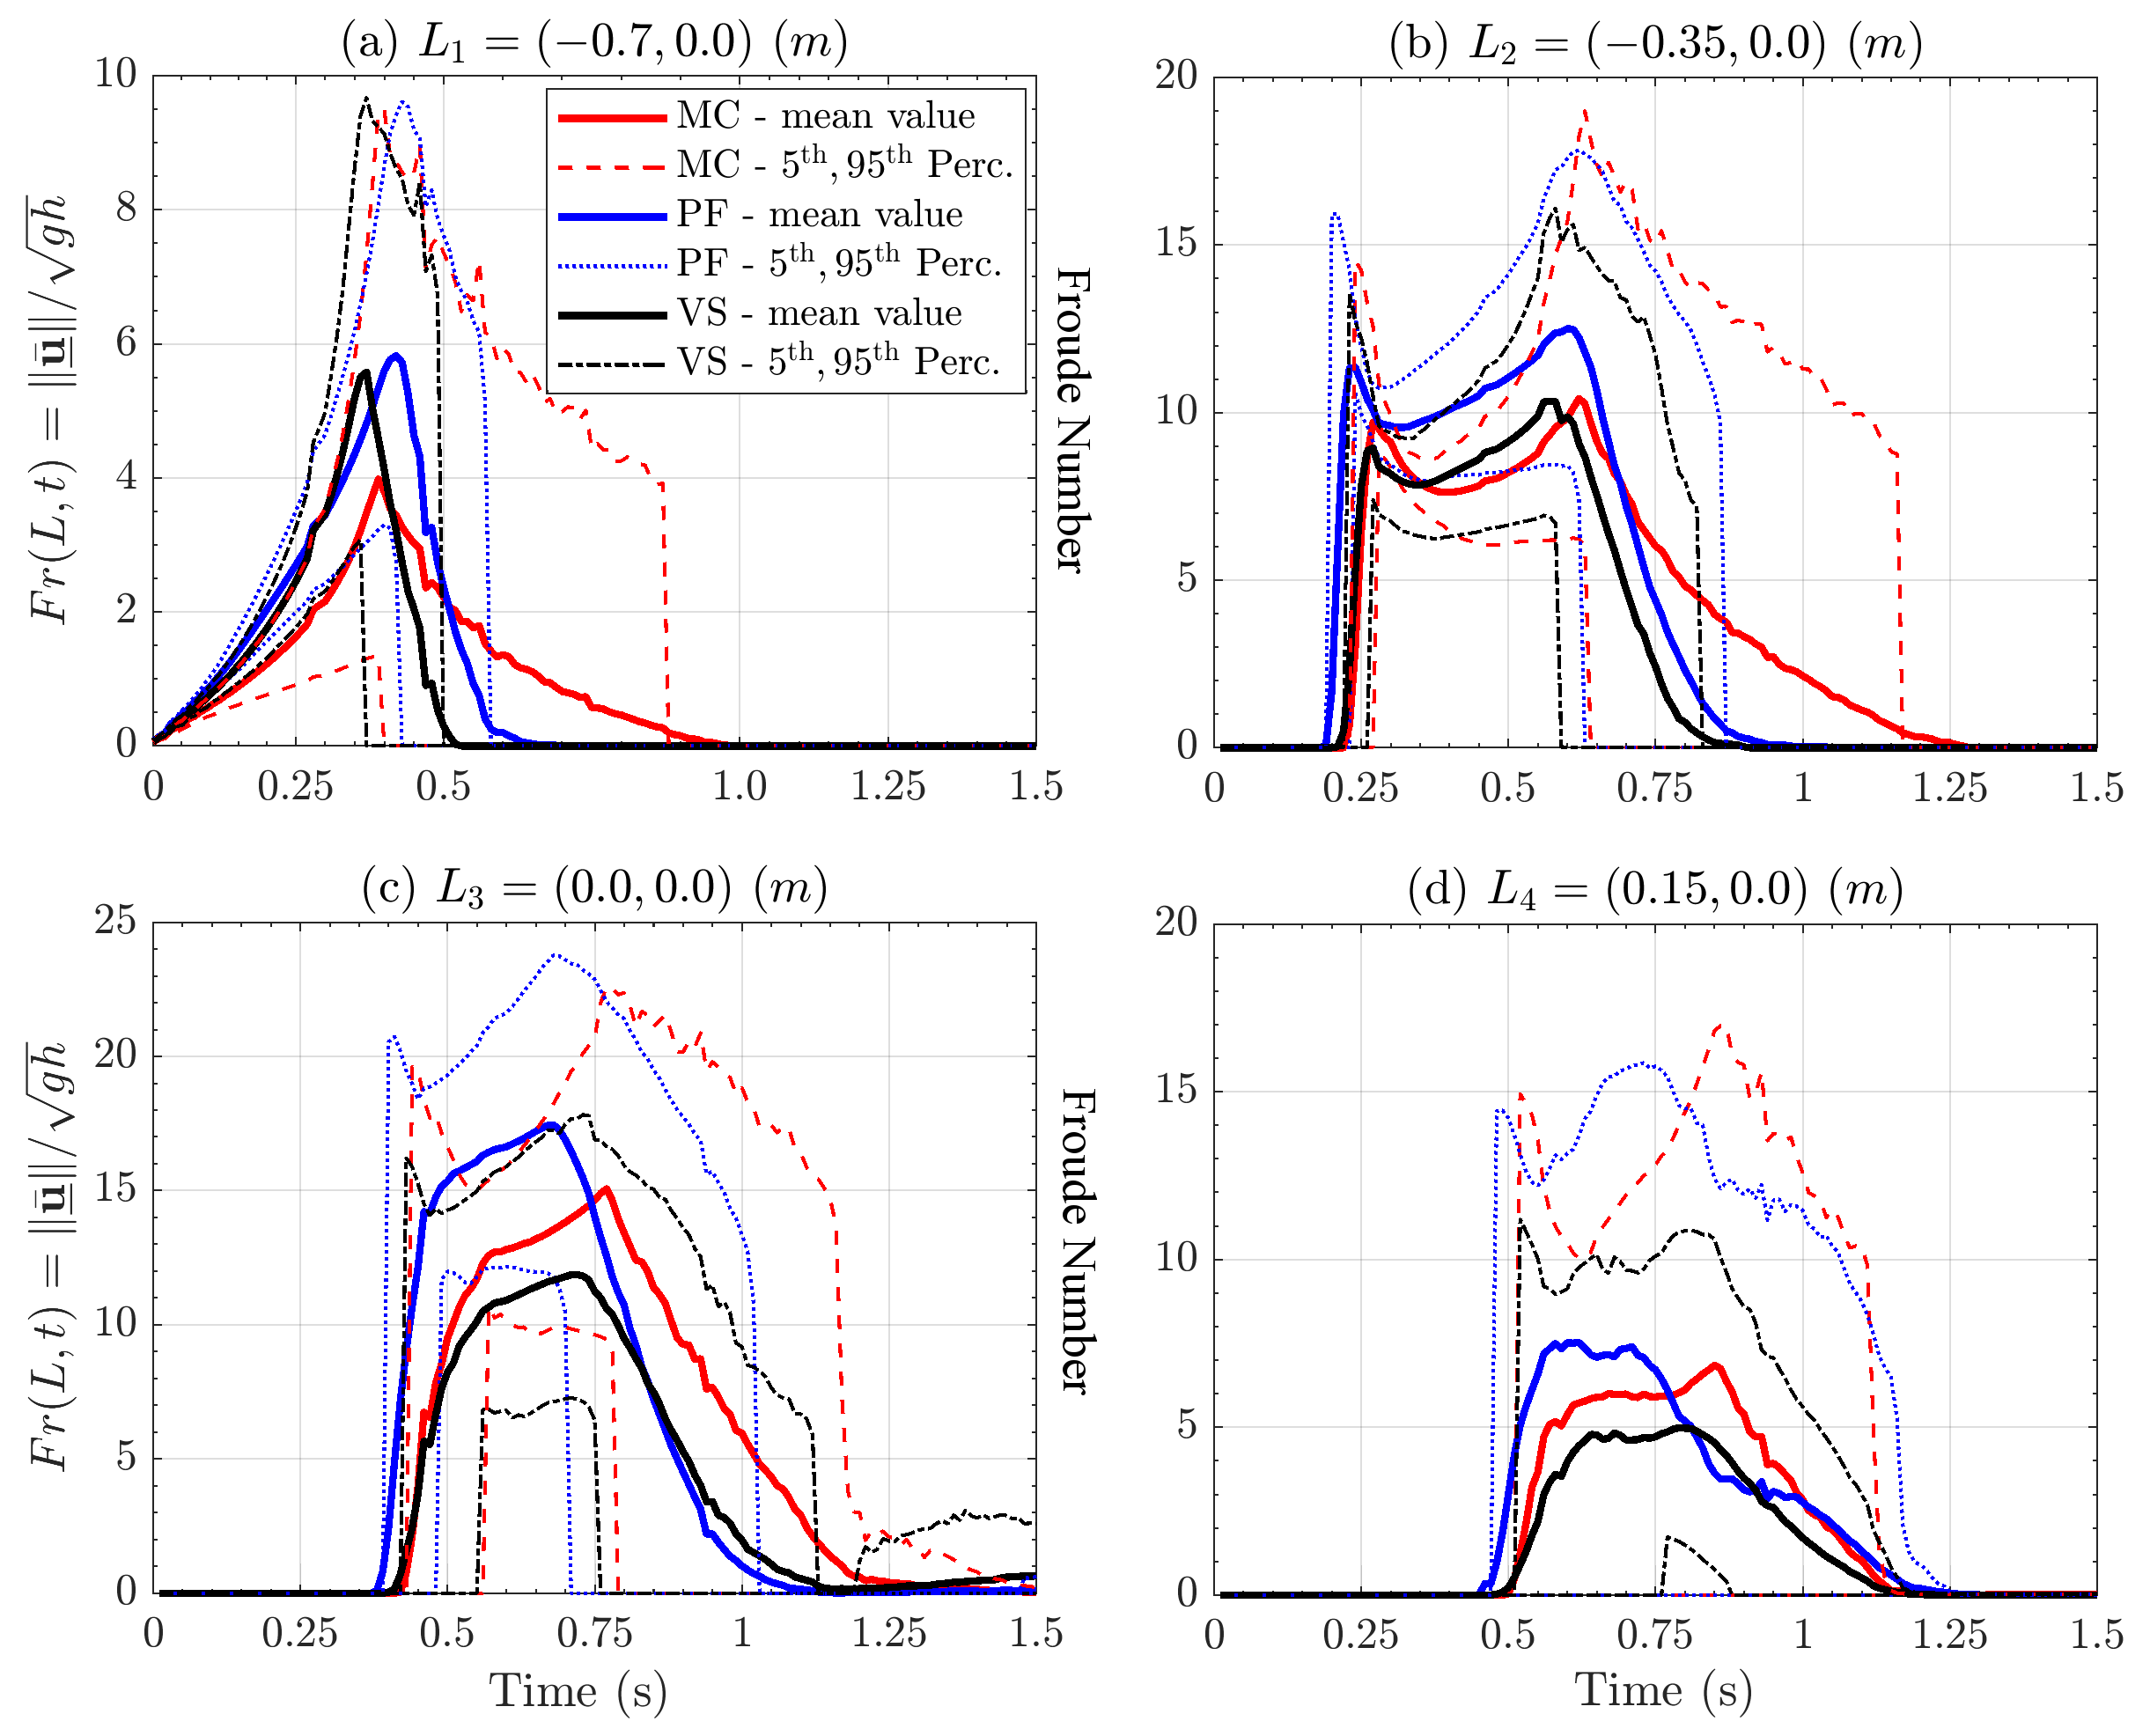
\includegraphics[width=0.9\textwidth]{InclinedPlane/LocalMeasurments/Froude.png}
        \caption{Froude number at four spatial locations. Bold line is mean value, dashed/dotted lines are 5$^{\mathrm{th}}$ and 95$^{\mathrm{th}}$ percentile bounds. Different models are displayed with different colors.}
        \label{fig:Ramp-Fr}
\end{figure}
Froude Number combines the estimates of flow height and speed. In plot \ref{fig:Ramp-Fr}a, related to point $L_1$, $Fr$ maximum average value is smaller for the MC model, $\sim 4$, than for the others, $\sim 6$. However, UQ tells us that 95$^{\mathrm{th}}$ percentile almost reaches $\sim 10$ in all the three models. After the peak, the values decrease slower and more concavely in MC model than in the others. In plot \ref{fig:Ramp-Fr}b, related to point $L_2$, $Fr$ shows a bimodal profile in time, with two separate peaks at $\sim 10$ on average, but reaching $\sim 18$ in the 95$^{\mathrm{th}}$ percentile plot. In fact, first maximum, at $\sim 0.25$ s is due to the speed peak, and second, at $\sim 0.6$ s is related to $\sqrt{h}$ decreasing while the speed is not significantly changing. In plot \ref{fig:Ramp-Fr}c and \ref{fig:Ramp-Fr}d, related to points $L_3$ and $L_4$, bimodality is less accentuated and becomes a plateau profile in $\sim [0.5, 0.75]$ s. PF model gives significantly larger $Fr$ values, even $>20$ at $L_3$, due to a larger speed and a thinner flow. It is worth noting, for the sake of PF model, that $Fr>\beta$ and the flow is in the dynamic regime during the most of the time.

\subsection{Spatial integral of force terms}
Figure \ref{fig:Ramp-Fx-spatial} shows the spatial integral of the force terms in the slope direction. The spatial integration is performed on half spatial domain, due to the symmetry with respect to the flow central axis. In plot \ref{fig:Ramp-Fx-spatial}a $\boldsymbol{RHS_1}$ starts with a plateau at $\sim 1.3 N$ before $\sim 0.55 s$, then decreases to zero after the material crosses the change in slope. The force values are consistent with the expression $\rho \left(V/2\right) g_x$, representing half the weight of material, projected along the slope direction. Uncertainty range of $\pm 0.2 N$ on the peak values. MC decreases slower, and is affected by a more significant uncertainty after the change in slope. PF decreases faster. In plot \ref{fig:Ramp-Fx-spatial}b $\boldsymbol{RHS_2}$ is negative and opposed to the gravity. A similar profile is shared by the three models, with a first short-lasting weakening before $\sim 0.1 s$, a plateau with a small strengthening after $\sim 0.5 s$, and a final waning after $\sim 1 s$, at the conclusion of the dynamics. MC does not reach zero, while the other models do. VS values are generally $\sim 0.5 N$ weaker than MC, and PF is intermediate, except in the initial peak, where it is the weakest. Strongest forces are reached during the plateau, and are $\sim -0.55 N$, $\sim -0.75 N$, $\sim -0.9 N$, with uncertainty range of $\pm 0.25 N$ in the plateau. Uncertainty is reduced in the final stages of VS and PF, but increases in MC. In plot \ref{fig:Ramp-Fx-spatial}c $\boldsymbol{RHS_3}$ is above zero only at the change in slope. It is always negative, i.e. reducing flow velocity, indeed it is equivalent to the friction due to the additional weigh generated by centrifugal forces. Its scale is ten times smaller than the previous plots, with values above $0.1 N$ only in MC. VS displays a bimodal profile, with a second and weaker peak at $\sim 0.75 s$. In plot \ref{fig:Ramp-Fx-spatial}d $\boldsymbol{RHS_4}$ is related to the additional forces of the models, differently characterized. In MC and PF, they are significantly small forces before $0.1 s$, completely negligible later. In VS, this is the velocity dependent term. It is negative and plays a significant role. It reaches $\sim 1 N$ at the change in slope, with uncertainty $\pm 0.3 N$. It is bell shaped and null before $\sim 0.1 s$ and after $\sim 1 s$.
\begin{figure}[H]
        \centering
        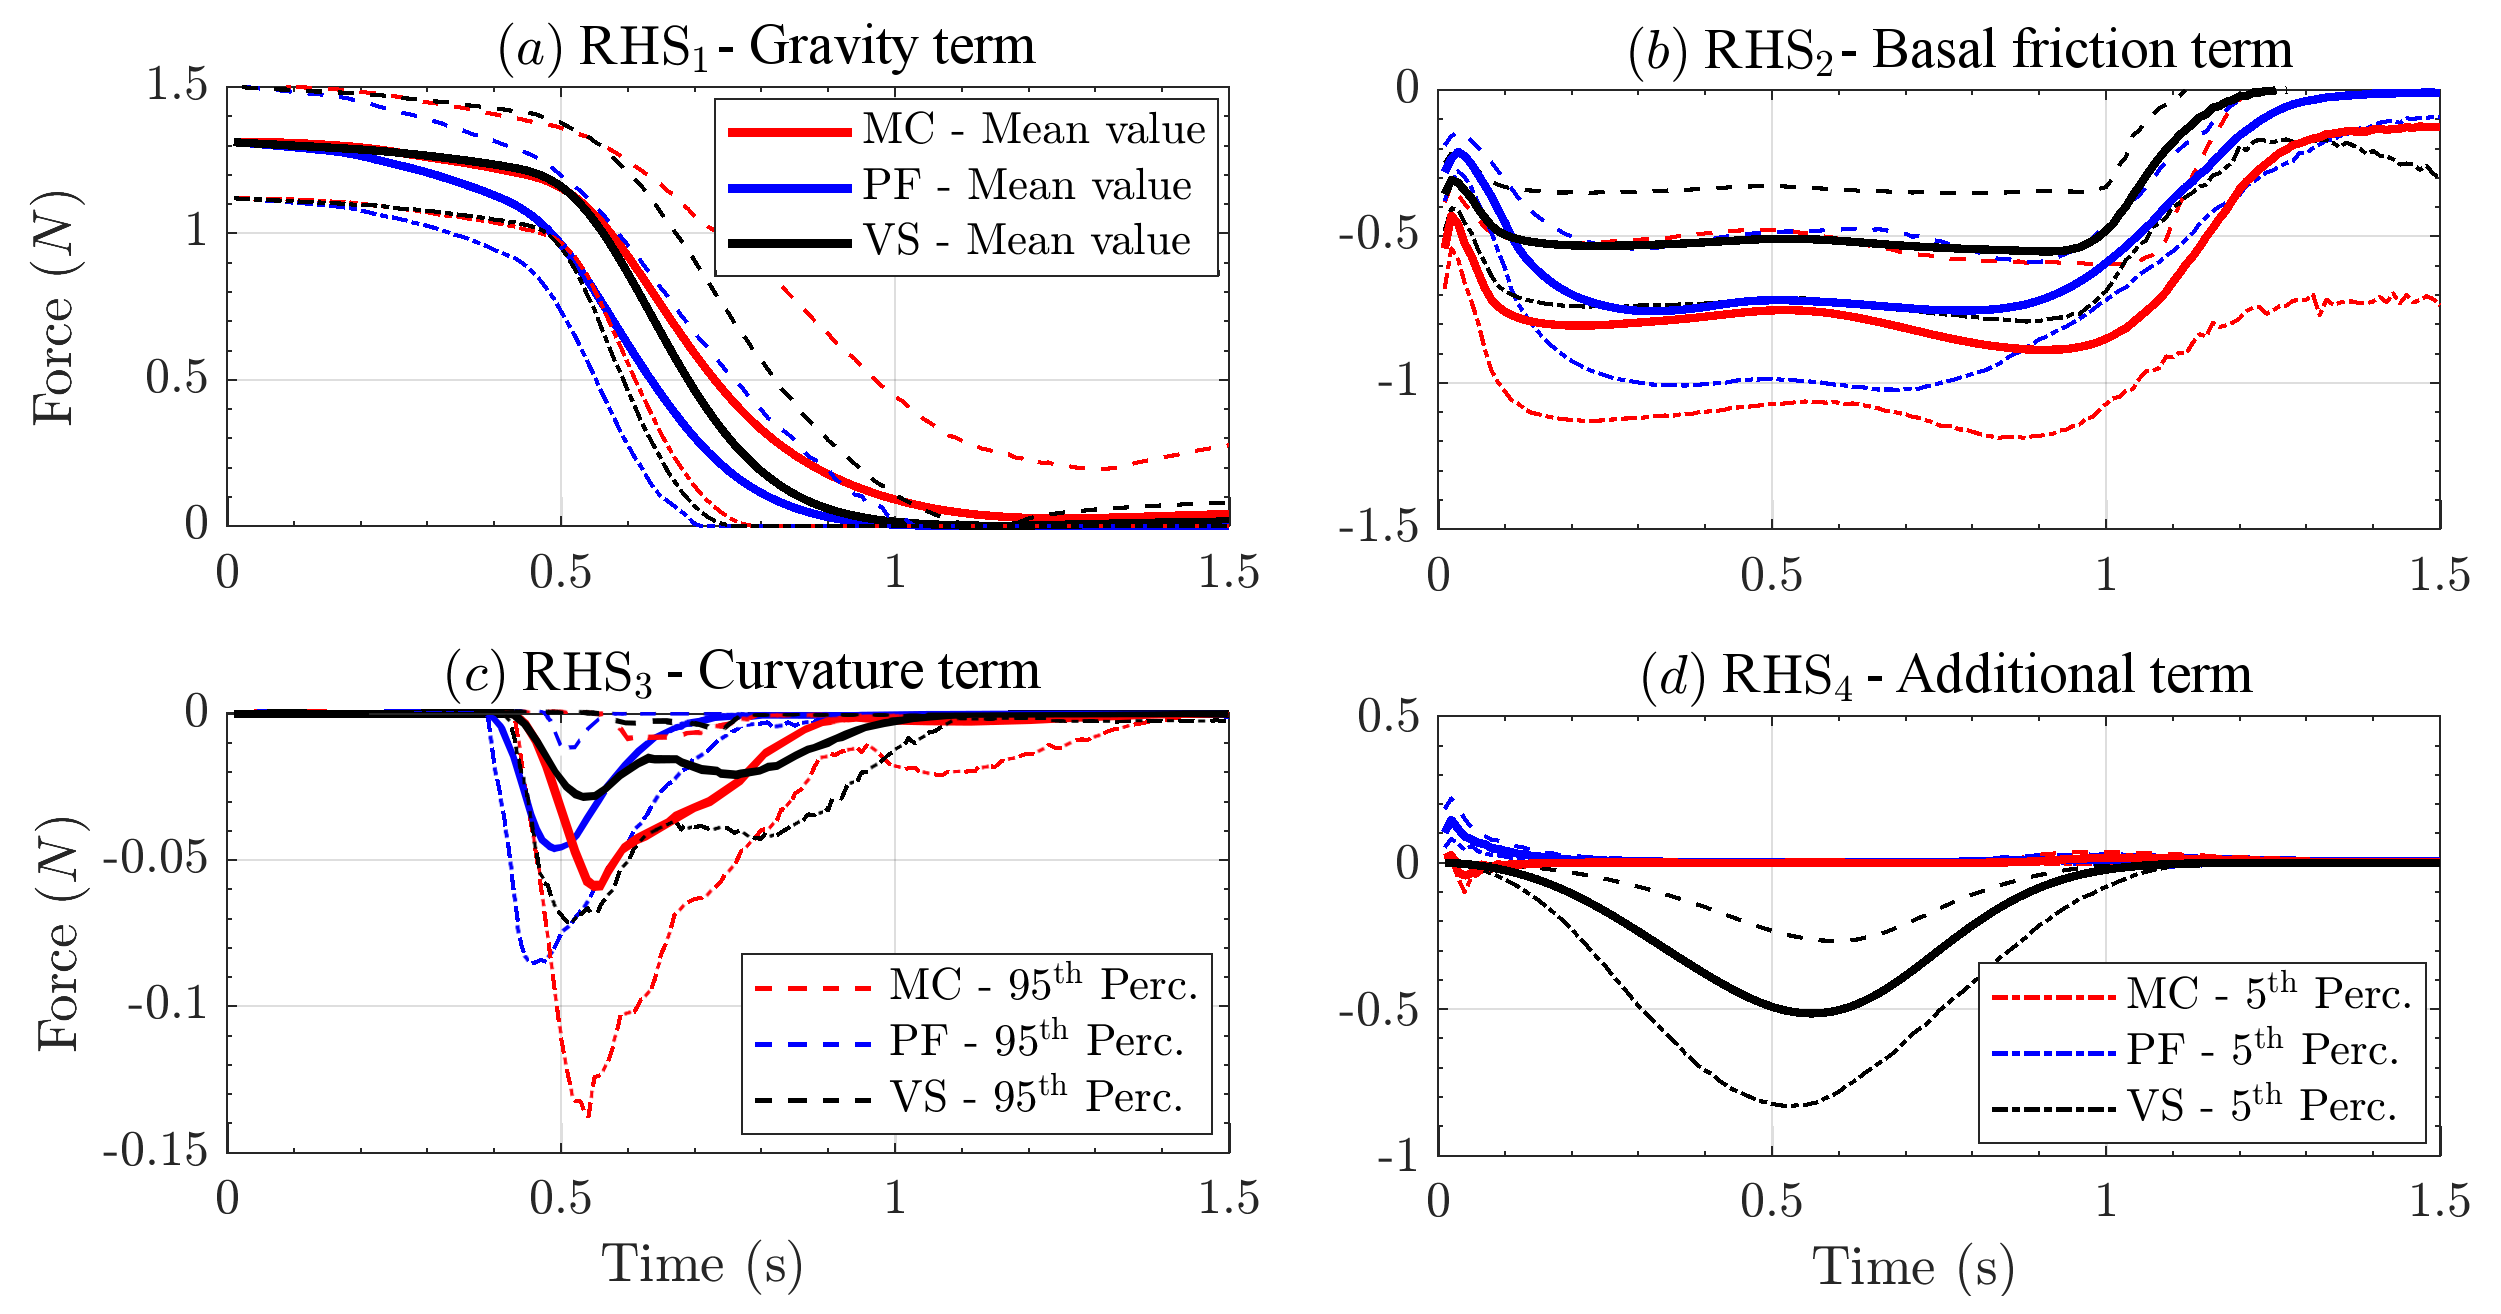
\includegraphics[width=0.95\textwidth]{InclinedPlane/AveragedMeasurments/ForcesIncline.png}
        \caption{Spatial integral of the RHS forces in the slope direction. Bold line is mean value, dashed lines are 5$^{\mathrm{th}}$ and 95$^{\mathrm{th}}$ percentile bounds. Scale of plot (c) is ten times larger than in (a),(b),(d).}
        \label{fig:Ramp-Fx-spatial}
\end{figure}
\newpage
\section{Large scale flow on the SW slope of Volc{\'a}n de Colima}
\subsection{Froude Number}
Figure \ref{fig:BAF-Fr-MC} shows an overview of the mean Froude Number, $\Vert \underline{\mathbf{u}} \Vert/\sqrt{gh}$, at the 51 spatial locations of interest, according to MC.
\begin{figure}[H]
         \centering
        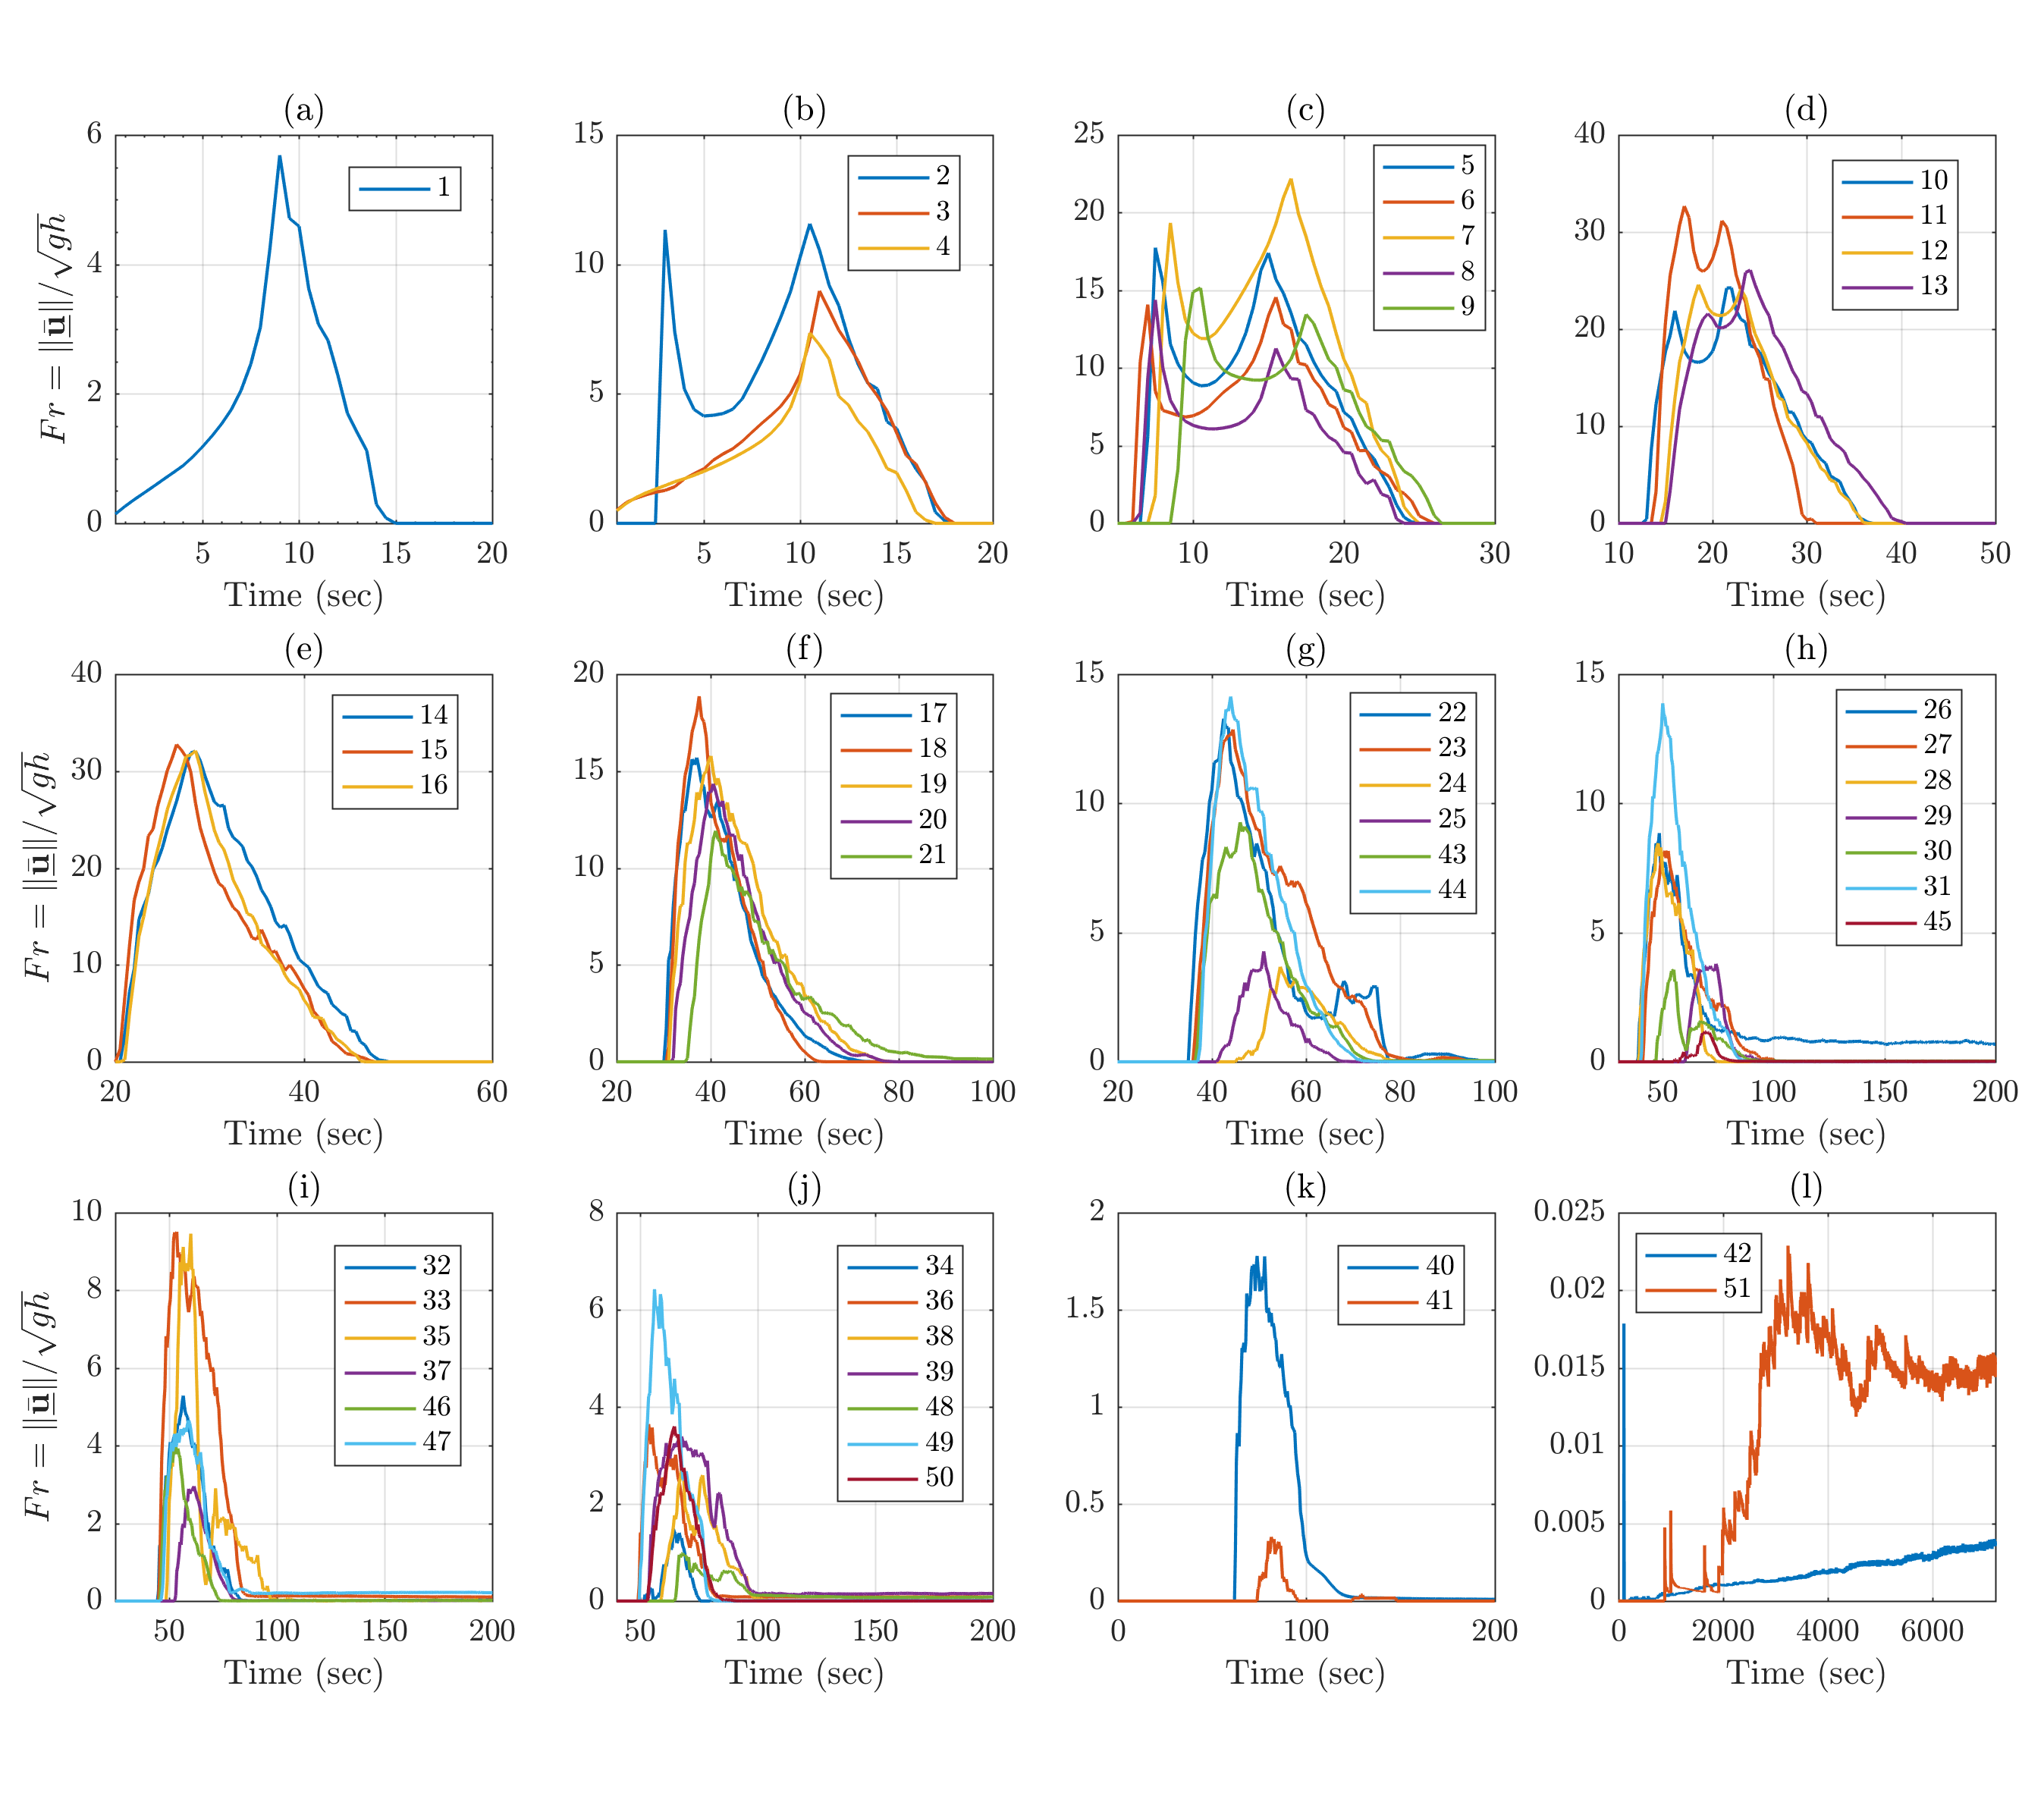
\includegraphics[width=0.9\textwidth]{MC&VS_51/Froude_MC2.png}
        \caption{MC model, records of average Froude Number in 51 numbered locations.}
        \label{fig:BAF-Fr-MC}
\end{figure}
Froude Number combines height and speed measurements, and plot profiles are similar to what observed in Figure \ref{fig:Ramp-Fr}. In particular, in plots \ref{fig:BAF-Fr-MC}b,c,d, a bimodal profile is observed due to the interplay between flow height and flow speed. In plots \ref{fig:BAF-Fr-MC}f,g,h,i,j, sharp changes are observed, and the plots are significantly rough when the speed is significantly small.
\newpage
Figure \ref{fig:Colima-Fr1} displays Froude Number, $\Vert \underline{\mathbf{u}} \Vert/\sqrt{gh}$, at the locations $(L_i)_{i=8,10,17,39,43,46}$. Froude Number is proportional on the ratio between the flow speed and the square root of flow height. Largest values are observed when the speed is significantly high compared to the flow height. Similarly to what observed in Fig. \ref{fig:Ramp-Fr} and \ref{fig:BAF-Fr-MC}, in plots \ref{fig:Colima-Fr1}a,b bimodal profiles are common. The first peak when the flow arrives in the location, the second when it leaves the location. Due to the slower dynamics of VS, the bimodal profile is less prominent. In PF the peaks, at $\sim 15$ and $\sim 30$, respectively, are slightly higher than in MC. In contrast, in plot \ref{fig:Colima-Fr1}c, MC displays an average Fr of $\sim 15$ significantly larger than in PF, $\sim 5$, and VS is almost null. In plot \ref{fig:Colima-Fr1}e the profile is similar, but with lower values. In plots \ref{fig:Colima-Fr1}d,f, only MC displays a not negligible Fr. The average is below $5$, but the 95$^{th}$ percentile can go above $20$.
\begin{figure}[H]
         \centering
        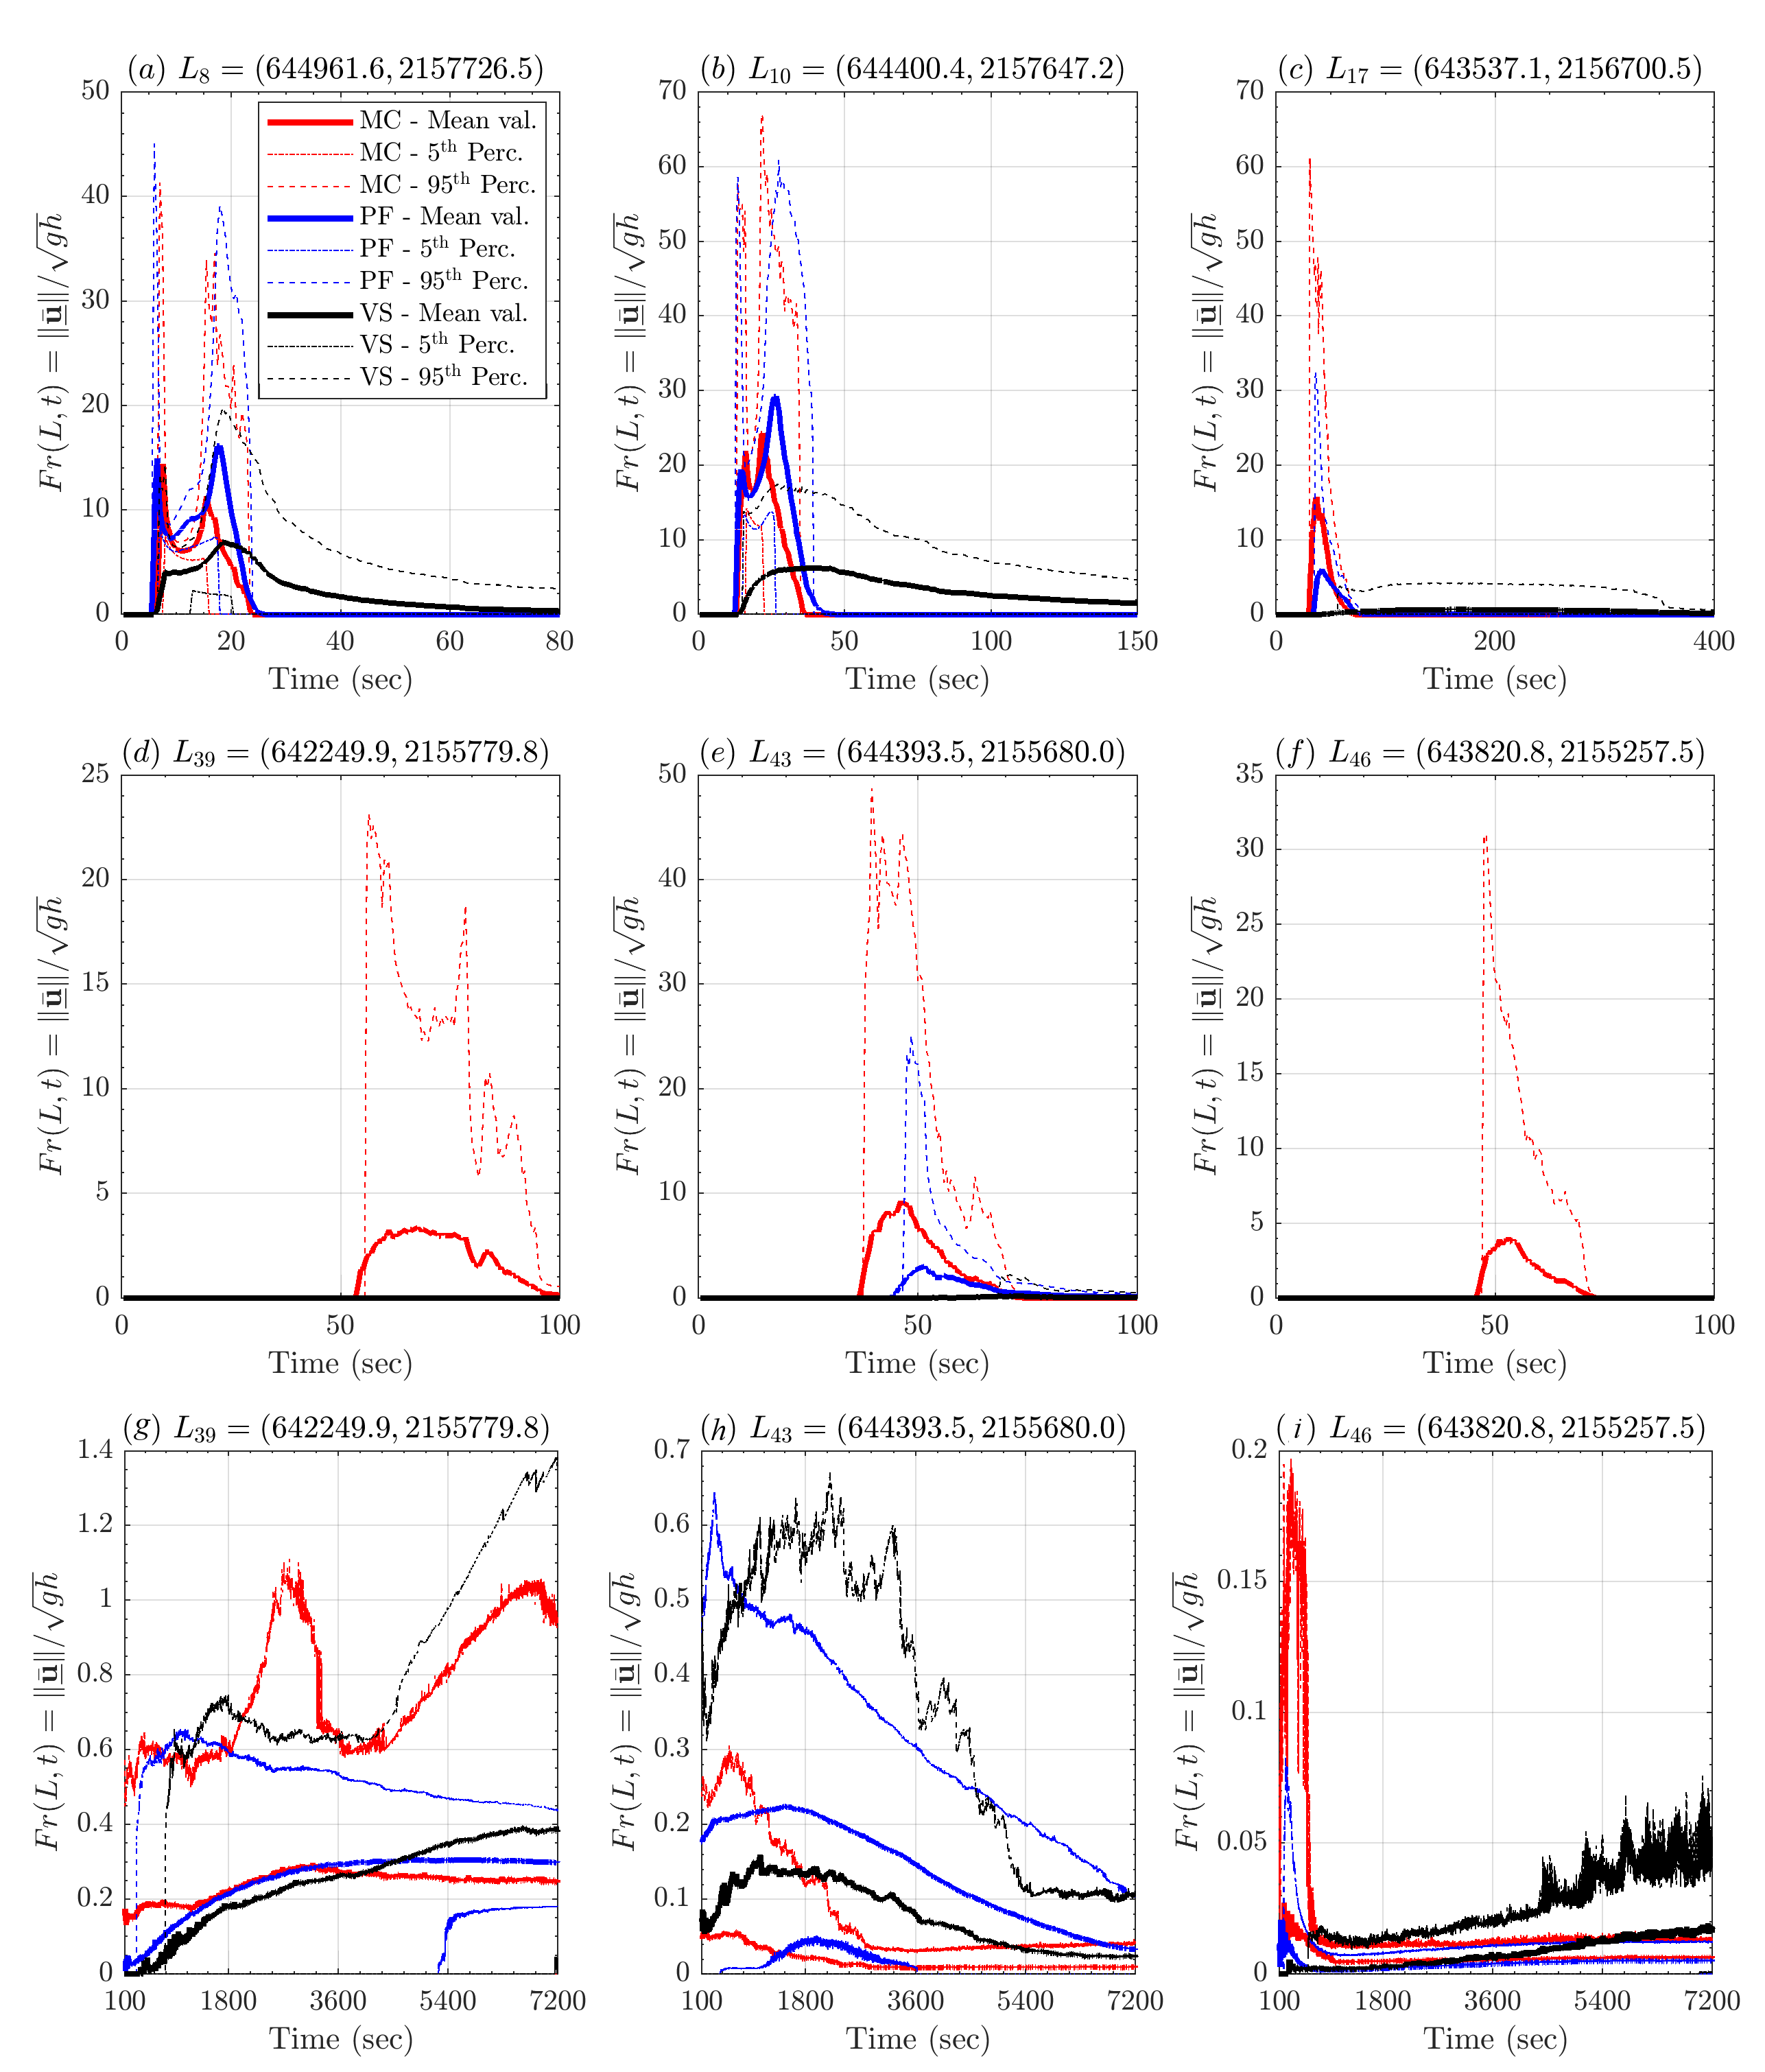
\includegraphics[width=1\textwidth]{BAF_VolcanDeColima/LocalMeasurments/Froude12.png}
        \caption{Records of Froude number at six selected locations. Bold line is mean value, dashed/dotted lines are 5$^{\mathrm{th}}$ and 95$^{\mathrm{th}}$ percentile bounds. Different models are displayed with different colors.}
        \label{fig:Colima-Fr1}
\end{figure}

\newpage
\subsection{Flow acceleration}
Figure \ref{fig:Colima-Accel1} shows the flow acceleration, $\Vert \underline{\mathbf{a}} \Vert(L,t)$, at the points $(L_i)_{i=8,10,17,39,43,46}$.
\begin{figure}[H]
         \centering
        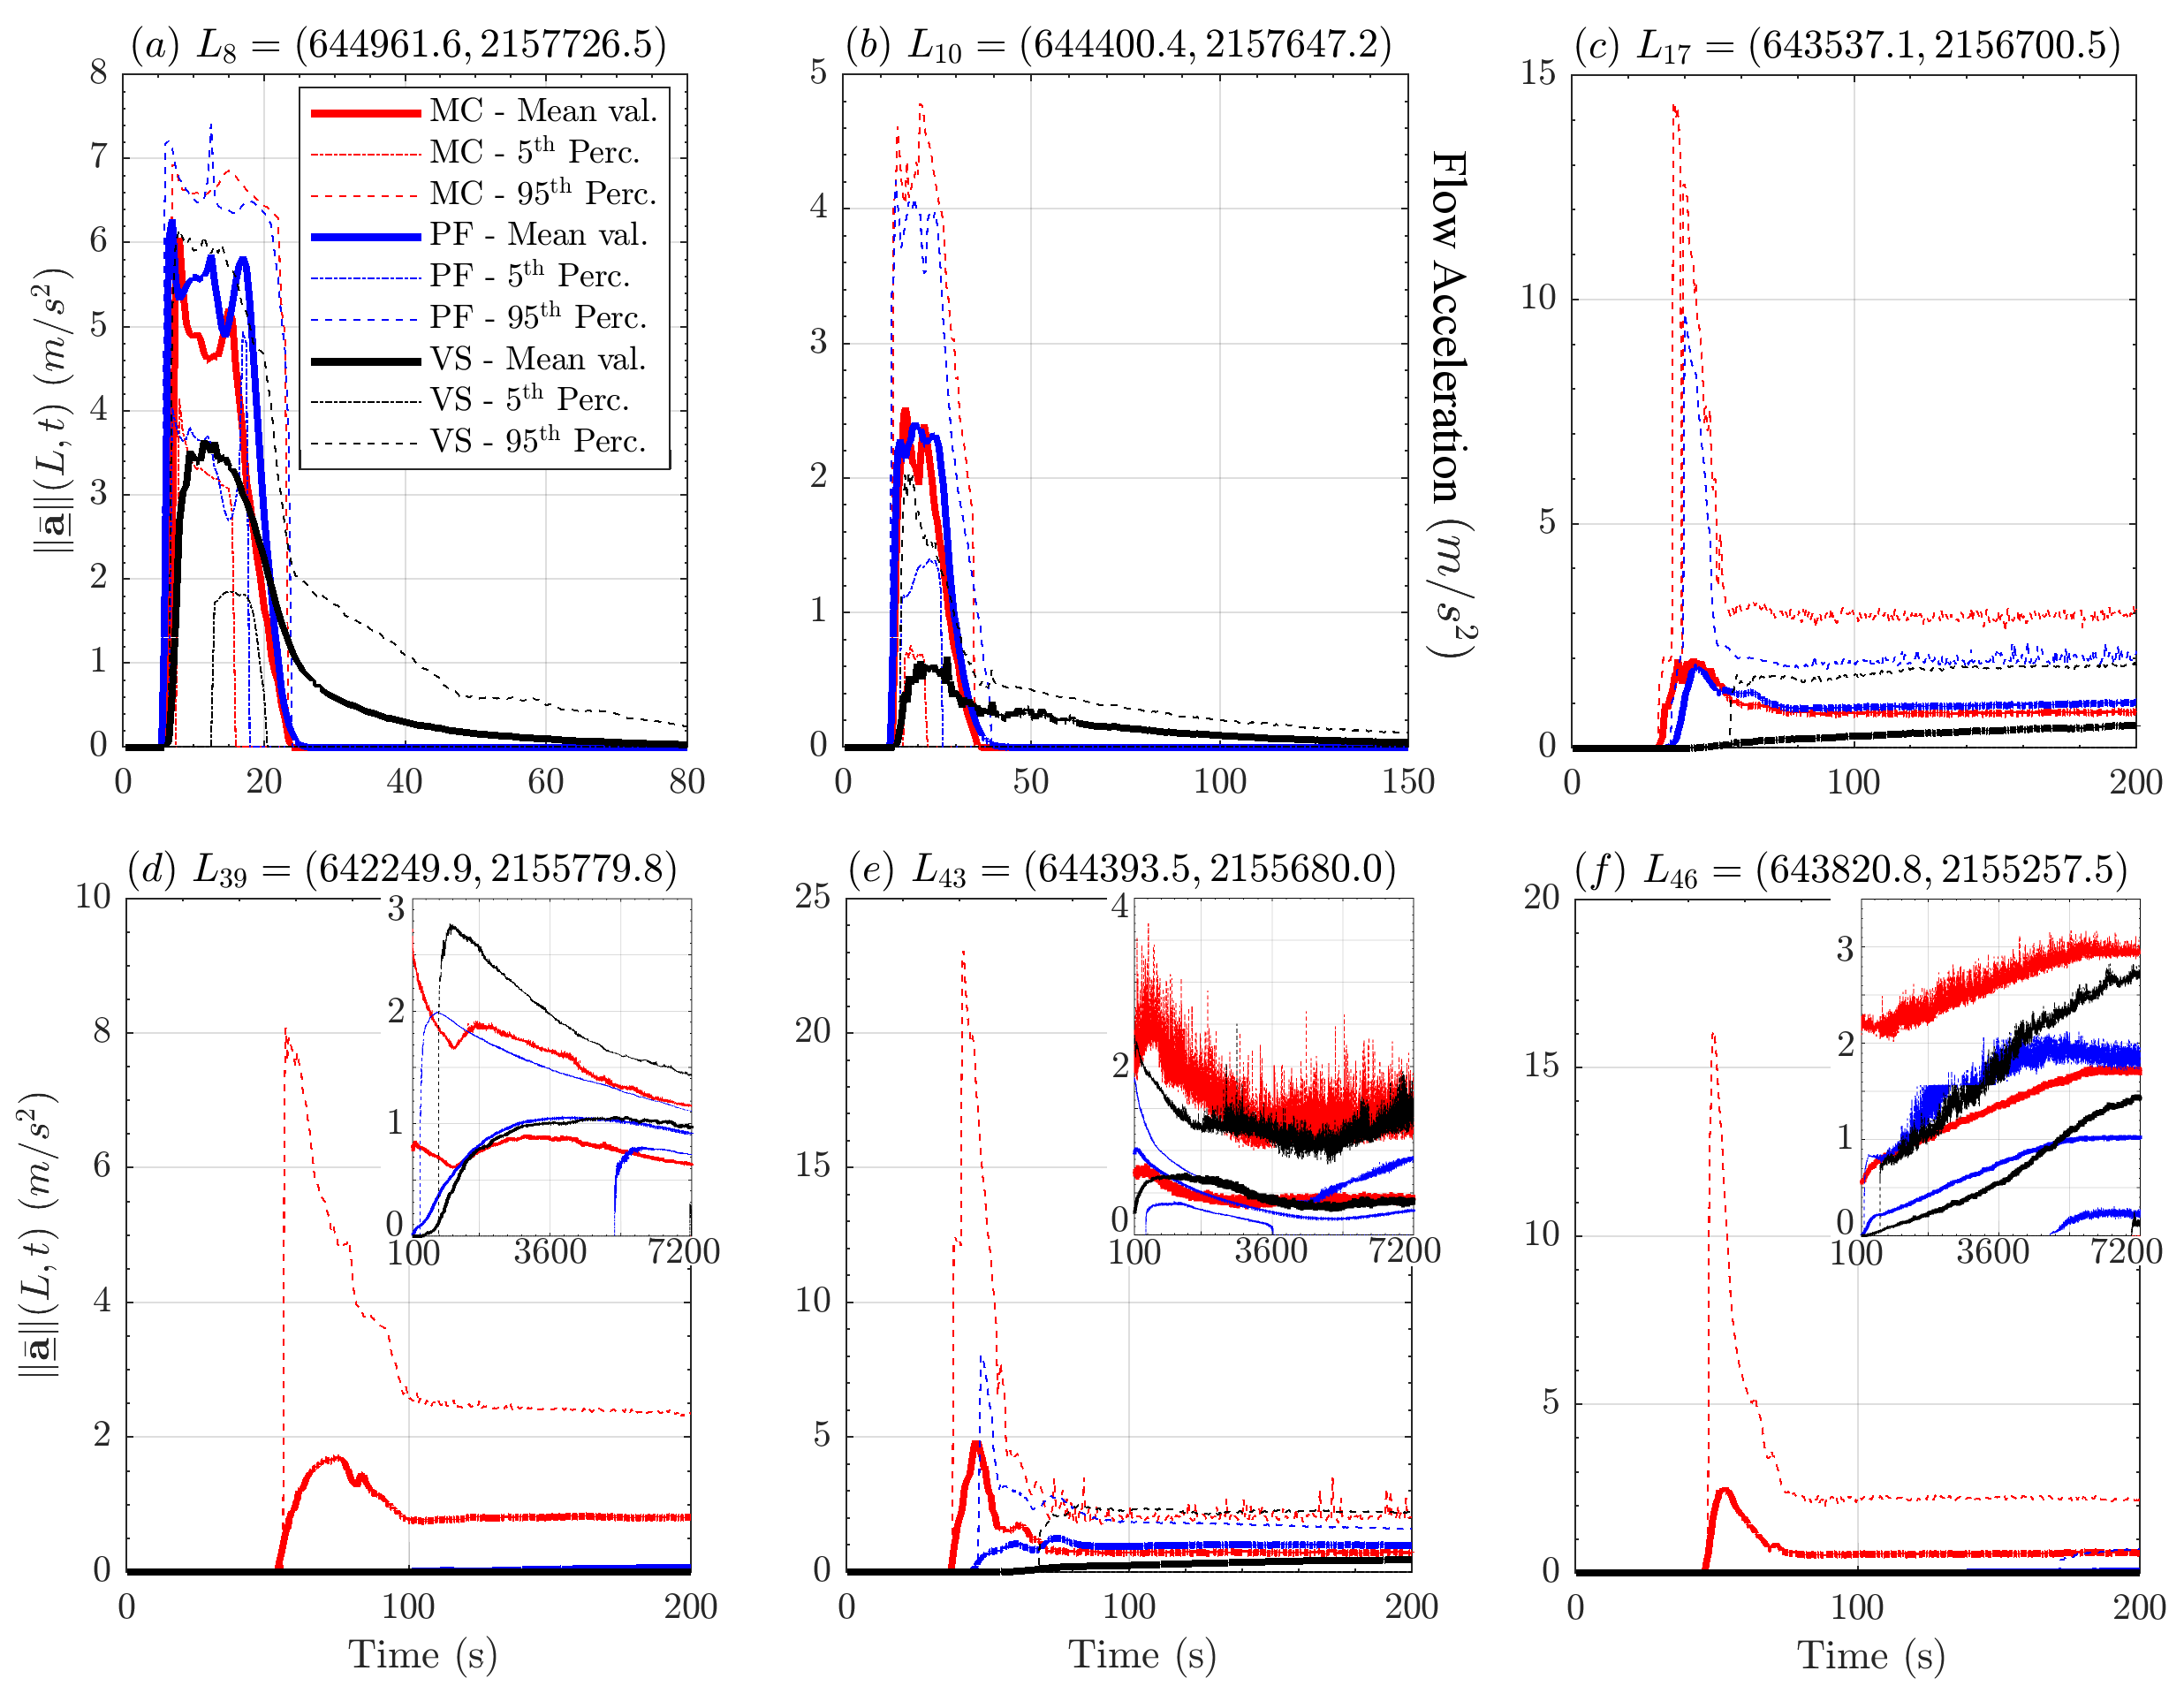
\includegraphics[width=1\textwidth]{BAF_VolcanDeColima/LocalMeasurments/Acceleration12.png}
        \caption{Flow acceleration in six numbered locations. Records of points $L_{39}$, and $L_{46}$ include small box with the asymptotic dynamics. Bold line is mean value, dashed lines are 5$^{\mathrm{th}}$ and 95$^{\mathrm{th}}$ percentile bounds. Different models are displayed with different colors. Numerical noise affecting percentile curves in the small box of (f) has been averaged.}
        \label{fig:Colima-Accel1}
\end{figure}
In plot \ref{fig:Colima-Accel1}a,b, MC and PF display a higher maximum acceleration, both at $\sim 6 m/s^2$ and $\sim 2.5 m/s^2$ in the first and second plot respectively, than VS, $\sim 3.5 m/s^2$ and $\sim 0.5 m/s^2$, respectively. The latter has a slower decrease to zero. Uncertainty in VS is more significant in plot \ref{fig:Colima-Accel1}a, than in plot \ref{fig:Colima-Accel1}b. It is the opposite in MC and PF. In plot \ref{fig:Colima-Accel1}c, in MC and PF there can be a significant peak in acceleration, up to $\sim 15 m/s^2$ and $\sim 10 m/s^2$, in the 95$^{th}$ percentile values, respectively. The same peak is absent in the average plots, which are significantly flat in all the models, displaying values at $\sim 1 m/s^2$ in MC and PF, and $\sim 0.5 m/s^2$ in VS, at $\sim 200 s$. Plot \ref{fig:Colima-Accel1}e is similar, but PF is lower and lacks of the peak in the 95$^{th}$ percentile values. In plot \ref{fig:Colima-Accel1}d,f, only MC shows significant acceleration values. Small plots display the acceleration values on a long time window of $7200 s$. The plots possess an increasing trend, with values up to $\sim 1 m/s^2$. In general, PF acceleration tends to be lower than in the other models.
\newpage
\subsection{Spatial integral of force terms}
Figure \ref{fig:Colima-F-spatial} shows the spatial sum of the force terms modulus.
\begin{figure}[H]
        \centering
        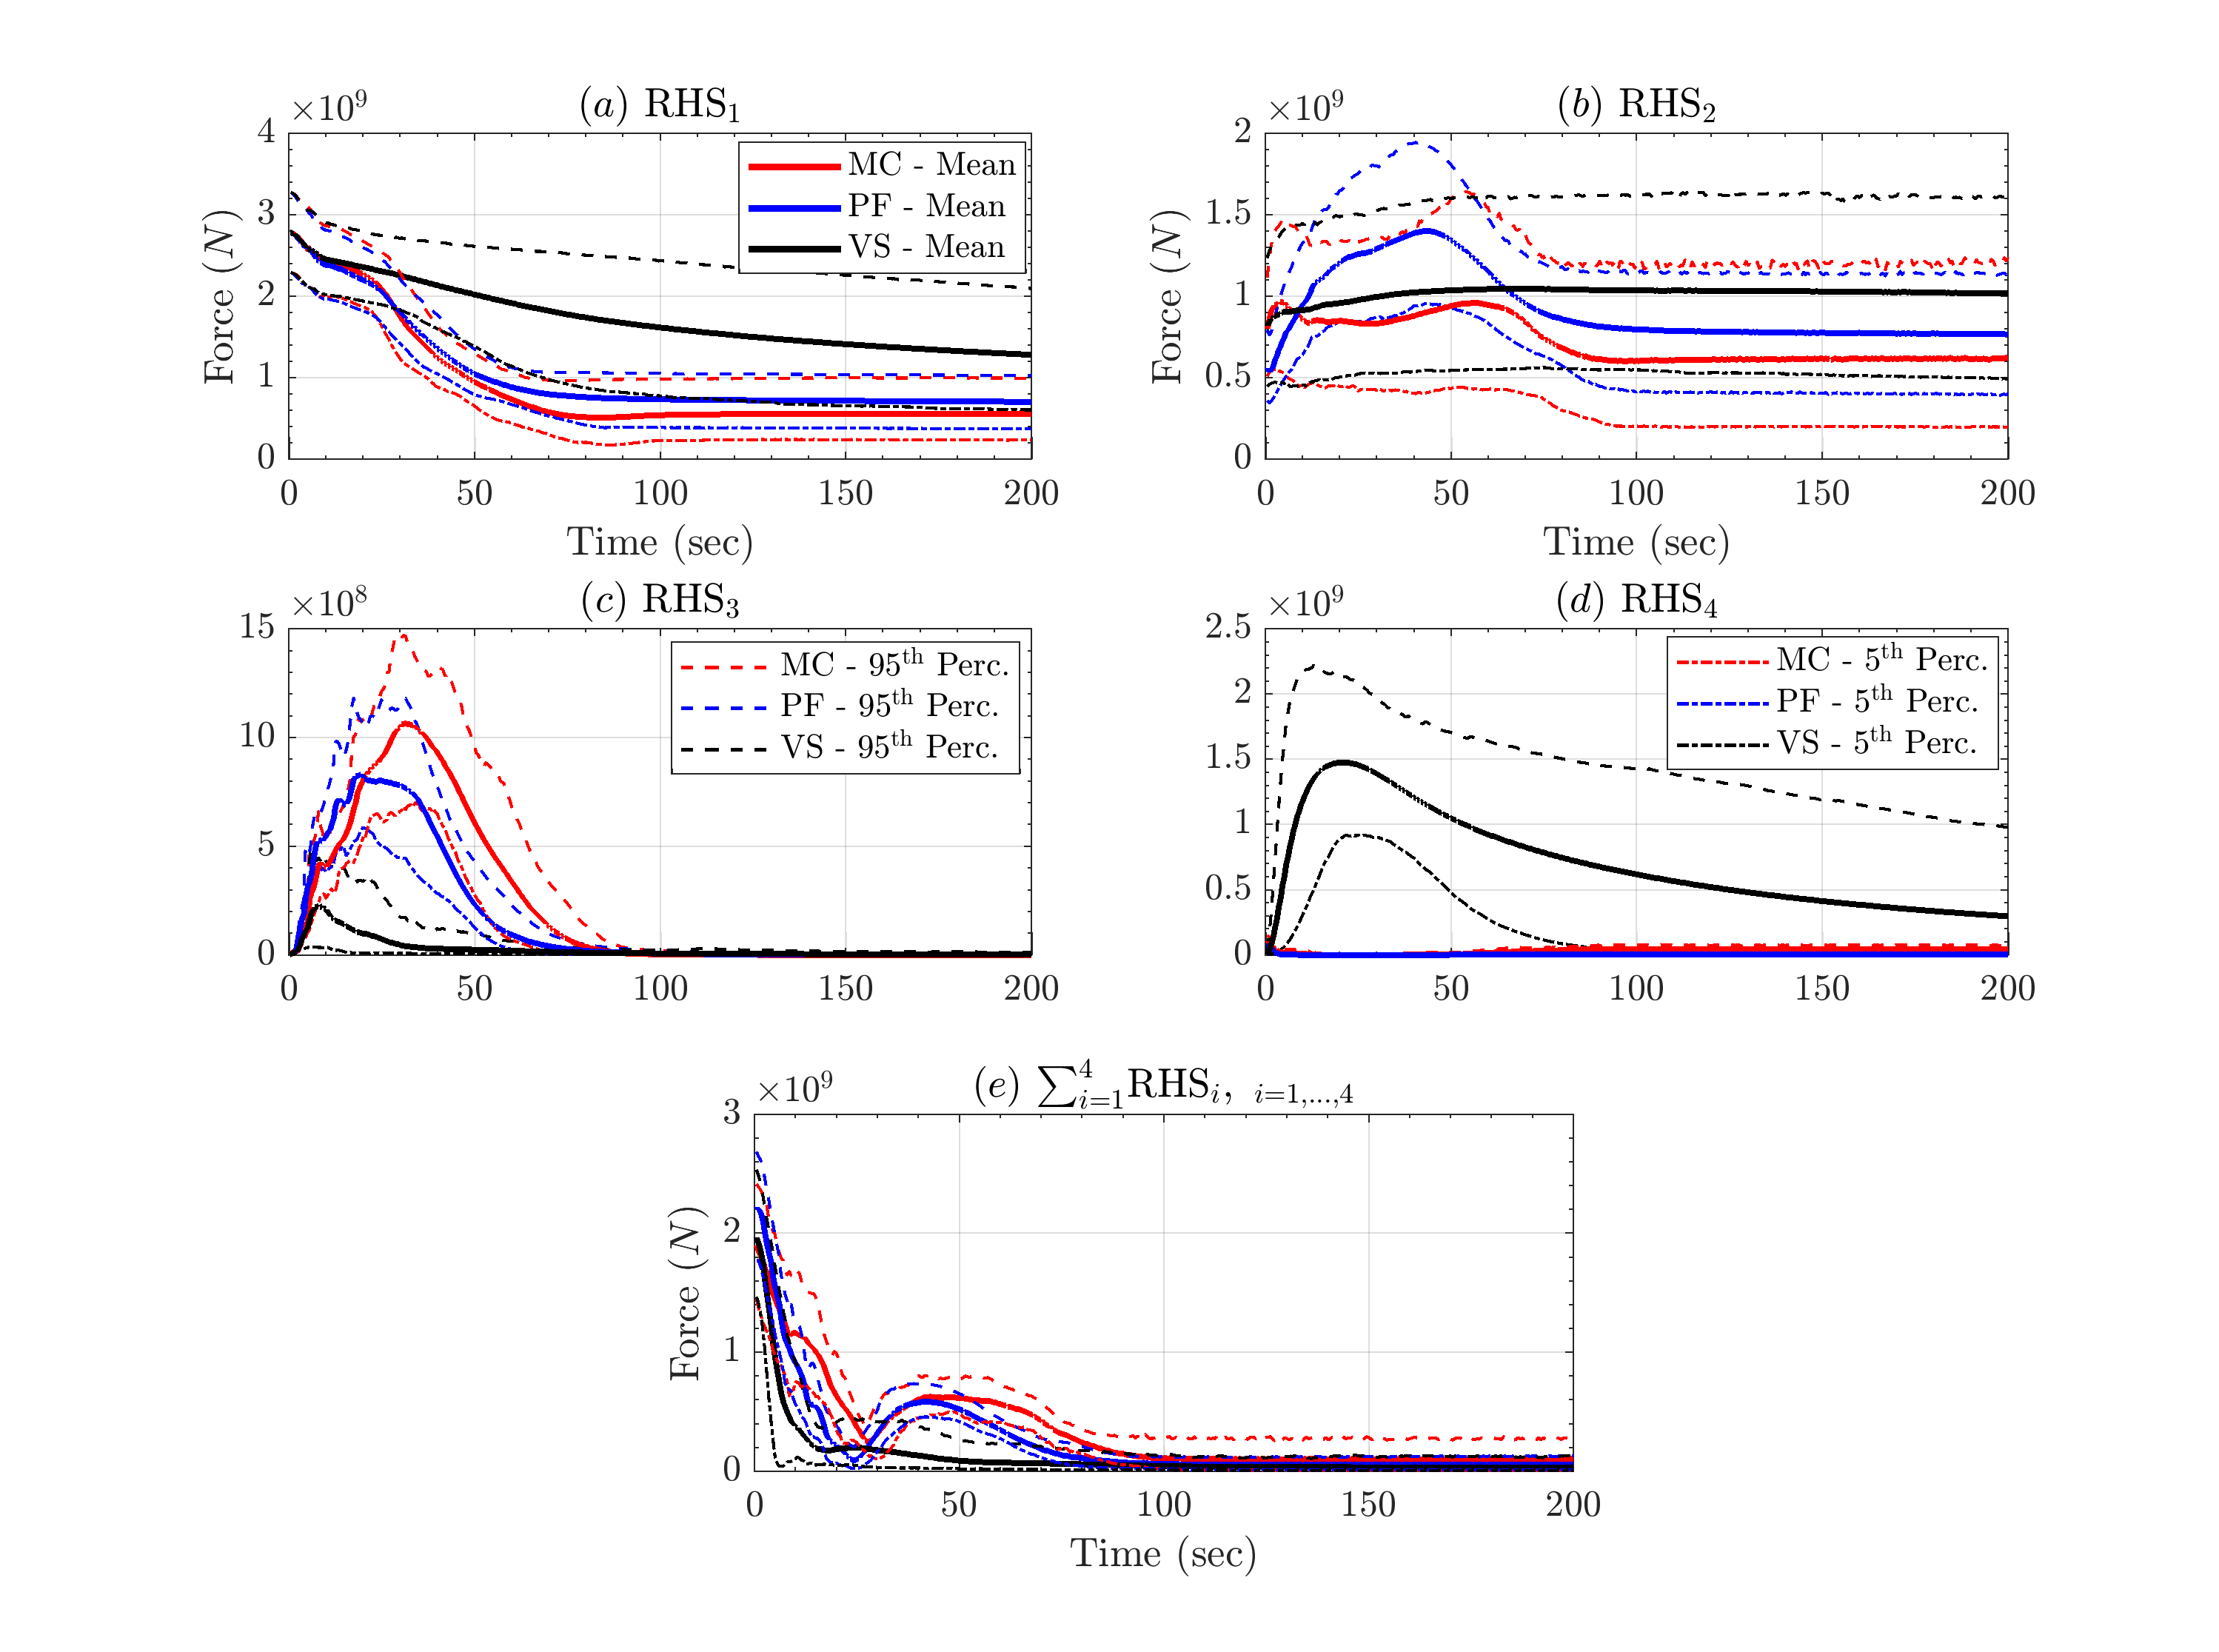
\includegraphics[width=0.95\textwidth]{BAF_VolcanDeColima/AveragedMeasurments/ForcesColima.png}
        \caption{Spatial integral of the RHS forces. Bold line is mean value, dashed lines are 5$^{\mathrm{th}}$ and 95$^{\mathrm{th}}$ percentile bounds. Different models are displayed with different colors.}
        \label{fig:Colima-F-spatial}
\end{figure}
The figure can be compared with Fig. \ref{fig:Ramp-Fx-spatial}. In plot \ref{fig:Colima-F-spatial}a $\boldsymbol{RHS_1}$ is decreasing, but more gradually in VS than in the others. Initial values are $2.8e9 N$ in all the models, uncertainty $\pm 2.5e8 N$. Force values are consistent with the material weight component along the mountain slope, and their decrease is related to the slope reduction. At $\sim 10 s$ all the models show a slowing down of the decrease, which is permanent in VS, and lasting $10 s$ in MC and PF. The latter models, reach a flat profile after $\sim 60 s$, at $6e8 N$ and $7e8 N$, respectively, and uncertainty of $\pm 2e8 N$ and $1.5e8 N$. VS, which flattens more gradually, is $1.3e9 N$ at $200 s$, uncertainty $[-7e8,+8e8] N$. In plot \ref{fig:Colima-F-spatial}b $\boldsymbol{RHS_2}$ shows a bimodal profile, with a peak at $5 s$, and a second one at $60 s$. Both of them at $9.5e8 N$ on average, with uncertainty of $[-4e8,+5e8] N$ in the first peak, and $[-5e8,+7e8] N$ in the second. The minimum between the two peaks is at $8e8 N$ and lasts from $10 s$ to $30 s$. After the second peak there is significant decrease, reaching $6e8 N$ at $90 s$, and becoming flat. Final uncertainty is $[-4e8, +6e8] N$. In PF, the plot starts from lower initial values than in the other models, but then has a unimodal peak of $1.4e9 N$ at $40 s$, on average. Uncertainty $\pm 5e8 N$. After that, the plot decreases, reaching $7.5e8 N$ at $90 s$, and becoming flat. Final uncertainty is $\pm 3.5e8 N N$, lower than in the other models. In VS, there is slow increase until the plot reaches $1.05e9 N$ at $70 s$. Then the average force is almost flat, at $1.0e9 N$, with significant uncertainty of $[-5e8,+6e8] N$. In plot \ref{fig:Colima-F-spatial}c $\boldsymbol{RHS_3}$ has a bell-shaped profile in all the models, waning to zero at $90 s$. However, MC reaches $1.1e9 N$ at $30 s$, PF $8e8 N$ at $20 s$, VS $2.5e8 N$ at $10 s$. The plot has a similar profile, but a different timing. The decrease is more gradual in VS. Uncertainty at the peak value is $\pm 4.5e8 N$ in MC, $[-2.5e8,+3.5e8] N$ in PF, $\pm 2e8 N$ in VS. In plot \ref{fig:Colima-F-spatial}d $\boldsymbol{RHS_4}$ has a different meaning in the three models. In MC it is the internal friction term, and it has a small peak in the first second, at $1e8 N$. After that it flattens to negligible values, but shows again values at $5e7 N$ after $60 s$. In PF it is the a depth averaged correction in the hydrostatic pressure, and has a almost negligible effect only in the first second, at $5e7 N$. In VS, instead, it is the velocity dependent term, and has a very relevant effect. The plot shows a bell-shaped profile, with a peak of $1.45e9 N$ at $20 s$. Uncertainty is $[-5.5e8, +6.6e8] N$, at the peak. After that, the force gradually decreases and is $3e8 N$ at $200 s$, on average. Uncertainty $[-3e8, +7e8] N$.
\end{document} 